% Это основная команда, с которой начинается любой \LaTeX-файл. Она отвечает за тип документа, с которым связаны основные правил оформления текста.
\documentclass{article}

% Здесь идет преамбула документа, тут пишутся команды, которые настраивают LaTeX окружение, подключаете внешние пакеты, определяете свои команды и окружения. В данном случае я это делаю в отдельных файлах, а тут подключаю эти файлы.

% Здесь я подключаю разные стилевые пакеты. Например возможности набирать особые символы или возможность компилировать русский текст. Подробное описание внутри.
\usepackage{packages}

% Здесь я определяю разные окружения, например, теоремы, определения, замечания и так далее. У этих окружений разные стили оформления, кроме того, эти окружения могут быть нумерованными или нет. Все подробно объяснено внутри.
\usepackage{environments}

% Здесь я определяю разные команды, которых нет в LaTeX, но мне нужны, например, команда \tr для обозначения следа матрицы. Или я переопределяю LaTeX команды, которые работают не так, как мне хотелось бы. Типичный пример мнимая и вещественная часть комплексного числа \Im, \Re. В оригинале они выглядят не так, как мы привыкли. Кроме того, \Im еще используется и для обозначения образа линейного отображения. Подробнее описано внутри.
\usepackage{commands}

% Здесь я настроил пакет listings для отображения кода C++. Можно пользоваться непосредственно самим пакетом listings, но если вы про него ничего не знаете, то моя надстройка будет удобной стартовой точкой.
\usepackage{code}

% Потребуется для вставки картинки подписи
\usepackage{graphicx}

% Пакет для титульника проекта
\usepackage{titlepage}

% Здесь задаем параметры титульной страницы
\setUDK{192.168.1.1}
% Выбрать одно из двух
%\setToResearch
\setToProgram

\setTitle{ПО для топологического анализа данных}

% Выбрать одно из трех:
% КТ1 -- \setStageOne
% КТ2 -- \setStageTwo
% Финальная версия -- \setStageFinal
%\setStageOne
%\setStageTwo
\setStageFinal

\setGroup{225}
% Сюда можно воткнуть картинку подписи с помощью \includegraphics[scale=0.2]{<имя файла>}
% (scale подбирается индивидуально для конкретной картинки)
\setStudentSgn{\includegraphics[scale=0.2]{1.png}}
\setStudent{С.А.Корняков}
\setStudentDate{29.04.2025}
\setAdvisor{Качан Олег Николаевич}
\setAdvisorTitle{-}
\setAdvisorAffiliation{Лаборатория ИИ Сбербанка}
\setAdvisorDate{}
\setGrade{}
% Сюда можно воткнуть картинку подписи с помощью \includegraphics[scale=0.2]{<имя файла>}
% (scale подбирается индивидуально для конкретной картинки)
\setAdvisorSgn{}
\setYear{2025}


% С этого момента начинается текст документа
\begin{document}

% Эта команда создает титульную страницу
\makeTitlePage

% Здесь будет автоматически генерироваться содержание документа
\tableofcontents
\newpage
% Данное окружение оформляет аннотацию: краткое описание текста выделенным абзацем после заголовка
\begin{abstract}
  Цель работы заключается в разработке библиотеки для топологического анализа данных, объединяющей современные алгоритмы построения симплициальных комплексов и вычисления персистентных гомологий. Основные задачи включают:
  \begin{itemize}
    \item Реализацию оптимизированных алгоритмов (\texttt{Twist}, \texttt{DoubleTwist}) для построения диаграмм устойчивости
    \item Вычисление гармонических представителей через ядро матрицы Ходжа-Лапласа
    \item Создание модульной архитектуры с поддержкой исследовательских модификаций
    \item Интеграцию современных структур данных (\texttt{BitTreeColumn}, оптимизированные деревья симплексов)
  \end{itemize}
  Библиотека предоставляет два режима работы: высокопроизводительный для бенчмаркинга и расширяемый для научных экспериментов. Эксперименты на реальных данных подтвердили преимущество новых алгоритмов над классическими подходами.

  \textit{Ключевые слова: топологический анализ, симплициальный комплекс, Вьеторис-Рипс, DoubleTwist, диаграмма устойчивости, параллельное вычисление, C++, матрица Ходжа-Лапласа, гармонические представители}
\end{abstract}
\section{Введение}

Современные задачи анализа данных в машинном обучении, вычислительной биологии и нейронауках требуют обработки высокоразмерных пространств. Традиционные библиотеки (GUDHI, PHAT), основанные на алгоритмах 2000-х годов, становятся неэффективны для работы с большими данными. На замену им приходят новые теории и алгоритмы, которые могут на порядок превосходить прежние алгоритмы по скорости.

Задача проекта заключается в создании библиотеки, которая реализует и комбинирует алгоритмы, собранные с множества новейших статей, для ускоренного и параллельного вычисления симплициальных комплексов, диаграмм устойчивости, ядра матрицы Ходжа-Лапласа и гармонических представителей. Библиотека имеет два направления:
\begin{enumerate}
  \item Оптимизированная под конкретные алгоритмы для наибыстрейшего вычисления. Это позволит сравнить данную имплементацию с другими библиотеками на скорость
  \item Модульная, с максимальным количеством шаблонов и абстракций. Данная версия необходима в научных и исследовательских целях для экспериментов над гипотезами. Она позволит быстро и удобно реализовывать нужные для исследований алгоритмы и объекты
\end{enumerate}

\subsection*{В поставленные задачи входило:}
\subsubsection*{Изучение теории}
Изучена теория симплициальных комплексов, гомологических групп, диаграмм устойчивости, матрицы Ходжа-Лапласа на графах, гармонических цепей и циклов. Прочитаны реализованные в библиотеках алгоритмы для вычисления и построения этих объектов, а также исследованы новейшие алгоритмы, которые пока не имеют общедоступных реализаций.
\subsubsection*{Реализация необходимых объектов}
Имплементированы на языке программирования C++ различные топологические объекты, нужные для вычисления гармонический циклов:
\begin{itemize}
  \item Облако точек
  \item Симплекс, фильтрованный симплекс
  \item Дерево симплексов для быстрого нахождения их позиций в отфильтрованном комплексе \autocite{simplextree}
    \begin{enumerate}
      \item Обычная реализация с провязыванием соседей с одинаковыми номерами вершин на одной высоте
      \item Оптимизированные версии, чтобы быстро работать с полным 2-скелетом
    \end{enumerate}
  \item Фильтрованный симплициальный комплекс
  \item Разреженная матрица позиций, представляющая граничную или кограничную матрицу фильтрованного комплекса
  \item Стоблец позиций для быстрого сложения во время редуцирования граничных/кограничных матриц
    \begin{enumerate}
      \item В виде обычного сета позиций
      \item В виде дерева битов \autocite{bittreecolumn}
    \end{enumerate}
  \item Диаграмма устойчивости
\end{itemize}

\subsubsection*{Имплементация алгоритмов}
Написаны следующие алгоритмы на полученных объектах:
\begin{itemize}
  \item Фильтрация облака точек для создания фильтрованного симплициального комплекса
    \begin{enumerate}
      \item Создание полного 2-скелета комплекса Вьеториса-Рипса
      \item Создание ограниченного по размерности и величине функции фильтрации комплекса Вьеториса-Рипса \autocite{new_vr}
    \end{enumerate}
  \item Создание граничной, кограничной и ориентированной граничной матриц фильтрованного симплициального комплекса.
  \item Редуцирование граничной матрицы фильтрованного симплициального комплекса:
  \begin{enumerate}
    \item Наивная реализация
    \item Параллельное редуцирование \autocite{parallelreduce}
    \item Twist \autocite{twist}
    \item DoubleTwist \autocite{doubletwist}
  \end{enumerate}
  \item Вычисление матрицы Ходжа-Лапласа \autocite{laplacianmatrix}
  \item Вычисление ядра разреженной матрицы
  \item Вычленение гармонического цикла из ядер матрицы Ходжа-Лапласа для различных позиций фильтрации
\end{itemize}

\subsubsection*{Абстрагирование алгоритмов и объектов}
Выделены модели объектов и алгоритмов, которые с помощью CRTP позволяет по-разному их реализовывать. Это позволило написать различные реализации одних и тех же действий, и с лёгкостью написать для них тесты, просто подменяя шаблонные параметры.

Данная абстрация позволила не разделять репозиторий на две ветки, а содержать все имплементации в одной и по запросу их использовать.

\subsubsection*{Тестирование библиотеки}
Тестирование проводилось с помощью фреймворка Catch2 \autocite{catch2}

Написаны юнит-тесты, стресс-тесты и тесты на корректность для всех объектов и алгоритмов. Используя синтетические и реальные данные, доказана корректность всех объектов и алгоритмов.

Для различных реализаций одних и тех же действий написаны бенчмарки, сравнивающие эти реализации, а также бенчмарки на масштабируемость.

Проведены сравнительные тесты с другими библиотеками и реализациями.

\subsubsection*{Изложение результатов}
В отчёте изложена теория, необходимая для понимания рассматриваемых алгоритмов и структур данных, а также описана архитектура и дизайн библиотеки. Написана сопроводительная документация для пользователей библиотеки.

\section{Требования к проекту}
\subsection{Функциональные требования}
Библиотека позволяет
\begin{enumerate}
  \item Считать облако точек из файлов разных форматов
  \item Построить фильтрованный симплициальный комплекс из облака точек
  \item Вычислить граничную/кограничную матрицы для фильтрованного комплекса
  \item Найти устойчивые пары фильтрованного комплекса
  \item Найти гармонические циклы фильтрованного комплекса
  \item Подменять реализацию объектов/алгоритмов
\end{enumerate}

\subsubsection{Модели}
Архитектура построена на принципах Generic Programming с использованием:
\begin{itemize}
  \item CRTP (Curiously Recurring Template Pattern) для статического полиморфизма
  \item Концепций \texttt{C++20} для валидации типов
  \item Policy-based design для замены компонентов
\end{itemize}

Большинство функций, методов и классов принимают не конкретные реализации, а модели объектов/алгоритмов, что делает код универсальным и открывает возможность добавлять эксперементальный функционал без трудностей.

Перечислим основные модели (а также их реализации, если их несколько):

\begin{itemize}
  \item Модель облака точек
  \item Модель фильтрации облака точек. Реализации:
  \begin{itemize}
    \item \texttt{NewVR} - фильтрация Вьеториса-Рипса с настраиваемым ограничением по радиусу и размерности симплексов \autocite{new_vr}
    \item \texttt{FullVR} - фильтрация Вьеториса-Рипса, которая строит полный 2-скелет
  \end{itemize}
  \item Модель дерева симплексов. Реализации:
  \begin{itemize}
    \item \texttt{SimplexTree} - классическое дерево симплексов \autocite{simplextree}
    \item \texttt{FullTree} - оптимизированное для полного 2-скелета дерево
  \end{itemize}
  \item Модель фильтрованного симплициального комплекса
  \item Модель матрицы инцидентности
  \item Модель кучи, которая имитирует исключающее "или" над позициями фильтрации. Реализации:
  \begin{itemize}
    \item \texttt{SetHeap} - позиции хранятся в сете
    \item \texttt{BitTreeHeap} - позиции хранятся в куче над вектором блоков \autocite{bittreecolumn}
  \end{itemize}
  \item Модель вычисления устойчивых пар из фильтрованного комплекса. Реализации:
  \begin{itemize}
    \item \texttt{Twist} — стандартная редукция граничной матрицы \autocite{twist}
    \item \texttt{DoubleTwist} — комбинированная редукция кограничной и граничной матриц \autocite{doubletwist}
  \end{itemize}
  \item Модель вычисления гармонических циклов из фильтрованного комплекса и его устойчивых пар
\end{itemize}
\subsection{Нефункциональные требования}
\subsubsection{Окружение программы}
\begin{enumerate}
  \item Программа написана на языке \texttt{C++}, используется версия языка \texttt{C++20}
  \item Для сборки и тестирования кода используется кросс-платформенная система сборки \texttt{CMake}
  \item Программа поддерживает множество компиляторов, но основной - \texttt{Clang}
  \item Проект использует систему поддержки версий \texttt{git} вместе с \texttt{github}
  \item Требуется не менее 32GiB RAM для корректной работы с большим объёмом данных
  \item Для форматирования используется \texttt{clang-format}
  \item Используется \texttt{clang-tidy} для унификации именований и статической диагностики программы
\end{enumerate}
\subsubsection{Используемые библиотеки}
\begin{enumerate}
  \item Библиотеки \texttt{Eigen} \autocite{eigen} и \texttt{Spectra} \autocite{spectra} для линейной алгебры над разреженными матрицами
  \item Библиотека \texttt{oneTBB} \autocite{onetbb} для параллелизации вычислений
  \item Фреймворк \texttt{Catch2} \autocite{catch2} для тестирования программы
\end{enumerate}
\subsubsection{Политика обработки ошибок}
\begin{enumerate}
  \item Исключения включены, но не бросаются самой библиотекой
  \item Вставлены \texttt{assert}-ы для выявления ошибок имплементации методов и алгоритмов
  \item Используется \texttt{std::optional} для обработки несуществования выходных данных алгоритмов и методов
\end{enumerate}
\section{Теория и описание алгоритмов}
{\smallДля ознакомления с основными понятиями см. раздел~\ref{glossary}}

Опишем объекты и алгоритмы по порядку:
\subsection{Фильтрация облака точек}
Опустим вырожденные случаи, а также ограничения на индексы, которые можно вывести из контекста.
\begin{definition}
  Пусть задано конечное множество вершин $V$. Симплициальным комплексом $K$ называется подмножество $2^V$, такое что:
  \begin{enumerate}
    \item Если $\sigma \in K$ и $\tau \subseteq \sigma$, то $\tau \in K$
  \end{enumerate}
  Тогда:
  \begin{itemize}
    \item Каждый элемент $\sigma \in K$ называется симплексом
    \item Симплекс $\sigma \in K$, состоящий $k+1$ вершин, называется $k$-симплекс и его размерность равна $\dim \sigma := k$
    \item Размерностью комплекса $\dim K$ называется максимальная размерность его симплексов
    \item $i$-скелетом комплекса $K$ называется $K^{(i)} := \{\sigma \in K\colon \dim \sigma \leq i\}$.
    \begin{example}
      $1$-скелет имеет структуру обычного графа с вершинами и рёбрами
    \end{example}
    \item Подкомплексом симплициального комплекса $K$ называется комплекс $K'\colon K'\subseteq K$. В частности, все $i$-скелеты комплекса являются его подкомплексами
\end{itemize}
\end{definition}

\begin{definition}
  Фильтрацией симплициального комплекса $K$ называется упорядоченное семейство симплициальных комплексов $\{K_f\}_{f \in A\subset \R}$, параметризованнное вещественным числом, такое что
  \[f_1 \leq f_2 \implies K_{f_1}\subseteq K_{f_2}\]
\end{definition}

\begin{definition}
Пусть задано конечное метрическое пространство $(M,\rho)$. Для заданного радиуса $r\in[0,\infty)$, комплекс Вьеториса-Рипса определяется как:
\[\mathbb{\rm{VR}}(M, r) = \{S \subseteq M \colon \forall v,u\in S\q \rho(v, u) \leq r\}\]
\end{definition}
Фильтрация Вьеториса-Рипса - это коллекция комплексов $\mathbb{\rm{VR}}(M, r)$:
\[\mathbb{\rm{VR}} = \{\mathbb{\rm{VR}}(M, r)\}_{r\in[0,\infty)}\]
Часто в топологическом анализе ограничивают $r \leq r_{max}$ и $|S| \leq d_{max} + 1$, чтобы работать только с $k$-скелетами комплексов.

Реализация фильтрации \texttt{FullVR} использует $r_{max} = \infty$ и $d_{max} = 2$, то есть просто строит полный 2-скелет. Но достаточно часто оказывается, что комплексы с радиусом больше некоторого порога не создают полезные гармонические циклы, а просто засоряют данные и замедляют вычисления. Поэтому был имплементирован новейший алгоритм \texttt{New-VR}, который позволяет эффективно строить такие фильтрации.

\subsubsection{New-VR}
Данный алгоритм использует несколько топологических наблюдений для ускорения построения фильтрации.
\begin{lemma}
  Пусть $\sigma_1, \sigma_2$ - два $k$-симплекса, и у них есть общая $(k-1)$-грань $\rho$. Пусть $v_i := \sigma_i \setminus \rho$. Если симплекс $\tau := \{v_0, v_1\}\in K$, то $\sigma_1 \cup \sigma_2$ является $(k+1)$-симплексом
\end{lemma}
\begin{definition}
  Пусть $K$ - симплициальный комплекс, и множество его вершин линейно-упорядочено. Тогда для каждой размерности $k$, мы введём лексикографический порядок для $k$-симплексов по порядку их вершин, т.е. $\sigma_1 < \sigma_2 \Leftrightarrow$ упорядоченный список вершин $\sigma_1$ лексикографически меньше упорядоченного списка вершин $\sigma_2$. 

  Аналогично введём порядок на парах различных $k$-симплексов:
  \[(\sigma_1 < \sigma_2) < (\tau_1 < \tau_2) \Leftrightarrow 
    \begin{cases}
      \sigma_1 < \tau_1\text{, or}\\
      \sigma_1 = \tau_1\text{ and }\sigma_2 < \tau_2\\
    \end{cases}\]
\end{definition}
\begin{lemma}
  Порядок выше задаёт линейно упорядоченное множество на парах различных $k$-симплексов.
\end{lemma}
\begin{theorem}
  Каждому $(k+1)$-симплексу соответствует ровно одна минимальная пара его $k$-граней и наоборот.
\end{theorem}
Данный факт позволяет при построении комплекса избегать дублирования симплексов и эффективно проверять только одно ребро для каждой пары $(\sigma_1 < \sigma_2)$.

Описание алгоритма создания фильтрации Вьеториса-Рипса из облака точек:
\begin{enumerate}
  \item Постройка графа смежности

    \begin{algorithm}[H]
    \caption{BuildAdjacencyGraph}
    \KwIn{Облако точек $P = [p_1,\dots,p_n]$, радиус $r_{max}$}
    \KwOut{Граф смежности $G$}
    $G \gets \varnothing$ \tcp{Инициализация пустого графа}

      \For{$u \in 1..n$}{
          \For{$v \in u+1..n$}{
            \If{$\rho(p_u, p_v) \leq r_{max}$}{
               $G[u] \gets G[u] \cup \{v\}$\;
            }
          }
      }
    \end{algorithm}
  \item Рекурсивное добавление кограней:

    \begin{algorithm}[H]
    \caption{NewAddCofaces}
    \KwIn{Текущий симплекс $\tau$, верхние соседи $N$, текущий радиус $r_{curr}$, фильтрация $F$, граф $G$}
    \KwOut{Обновлённая фильтрация $F$}
    $F \gets F \cup \{\tau, r_{curr}\}$ \tcp{Добавление симплекса $\tau$ в комплексы радиуса $\geq r_{curr}$}

    \If{$|\tau| > d_{max}$} {
      \Return
    }

    \For{$v \in N$} {
      $\sigma \gets \tau \cup \{v\}$

      $r_{new} \gets \max(r_{curr}, \q\max\limits_{u \in \tau} \rho(p_u, p_v))$

      $M \gets N \cap G[v]$ \tcp{Пересечение верхних соседей}

      \texttt{NewAddCofaces}($\sigma$, $M$, $r_{new}$, $F$, $G$)
    }
    \end{algorithm}

  \item Сам алгоритм можно выразить как

    \begin{algorithm}[H]
    \caption{NewVR}
    \KwIn{Облако точек $P = [p_1,\dots,p_n]$, радиус $r_{max}$, размерность $d_{max}$}
    \KwOut{Фильтрация F}
    $G \gets \text{\texttt{BuildAdjacencyGraph}($P$, $r_{max}$)}$

    $F \gets \varnothing$

    \For{$u \in 1..n$} {
      $\tau \gets \{u\}$

      $N \gets \{v \in G[u]\colon v > u\}$

      \texttt{NewAddCofaces}($\tau$, $N$, $0$, $F$, $G$)
    }
    \end{algorithm}
\end{enumerate}
\subsection{Диаграмма устойчивости}
Далее предполагаем, что вершины линейно-упорядочены.
\subsubsection{Гомологическая группа}
\begin{definition}
  Пусть $K$ - симплициальный комплекс, а $\Sigma_k$ - множество его $k$-симплексов. Тогда $k$-цепной группой $C_k(K)$ называется свободная абелева группа с базисом $B_k = \{[\sigma] \colon \sigma \in \Sigma_k\}$:
  \[C_k(K) := \left\{\sum_{i=1}^n a_i\sigma_i\right\}\]
  $k$-цепью называется элемент $k$-цепной группы. Обычно $a_i$ берут из поля $\Z_2$.
\end{definition}
\begin{definition}
  Граничным оператором $\delta_k \colon C_k(K) \to C_{k-1}(K)$ называется оператор, который отображает цепь $c = \sum a_i \sigma_i$ в:
  \[\delta_k(c) = \sum a_i \delta_k'(\sigma_i)\]
  где $\delta_k'$ отображает симплекс $\sigma:=[v_1,\dots,v_k]$ в
  \[\delta_k(\sigma) := \sum_{i=1}^k (-1)^{k-1} [v_1,\dots,\hat{v_i},\dots,v_k] \]
  где $\hat{v_i}$ означает удаление вершины $v_i$. 
\end{definition}
\begin{example}
Цепь $c := [v_1,v_2,v_3] - [v_2,v_3,v_5]$ отобразится в
\[\delta_3(c) = [v_2,v_3] - [v_1,v_3] + [v_1,v_2] - ([v_3,v_5] - [v_2,v_5] + [v_2,v_3]) = \]
\[=-[v_1,v_3] + [v_1,v_2] - [v_3,v_5] + [v_2,v_5]\]
\end{example}
С помощью данного оператора можно дать определения топологическим дыркам:
\begin{definition}
  Пусть $C_k(K)$ - $k$-цепная группа симплициального комплекса $K$. Тогда $k$-цепь $z\in C_k(K)$, для которой выполнено
  \[\delta_k(z) = 0\]
  называется $k$-циклом. Можно заметить, что множество всех $k$-циклов образуют ядро граничного оператора:
  \[Z_k(K) := \mathop{\rm Ker} \delta_k\]
\end{definition}
\begin{example}
  Цепь из рёбер $c := [v_1,v_2] + [v_2, v_3] - [v_1, v_3]$ образует цикл, если провести ориентированные рёбра между этими вершинами:
  \[\delta_1(c) = [v_2] - [v_1] + [v_3] - [v_2] - [v_3] + [v_1] = 0\]
\end{example}
\begin{definition}
  Пусть $C_k(K)$ - $k$-цепная группа симплициального комплекса $K$. Тогда $k$-границей называют $k$-цепь, которая является границей некоторой $(k+1)$-цепи, обозначим их:
  \[B_k(K) := \mathop{\rm Im} \delta_{k+1}\]
\end{definition}
\begin{lemma}
  $B_k(K)\subseteq Z_k(K)$, так как $\delta_k \circ \delta_{k+1} = 0$.
\end{lemma}
\begin{definition}
  Группа гомологий $H_k(K)$ называется факторгруппа
  \[H_k(K) := Z_k(K)/B_k(K)\]

  Элементы $H_k(K)$ называются классами гомологий. Два $k$-цикла называются гомологичными, если они принадлежат одному классу гомологий.
\end{definition}
\begin{example}
Классы гомологий можно представить как объединения всех способов описать дырку циклами. На рисунке~\ref{fig:homology_classes} дырку из 4 вершин описывают 3 разными циклами $z_1$, $z_2$ и $z_3$.
\begin{figure}[ht]
  \centering
  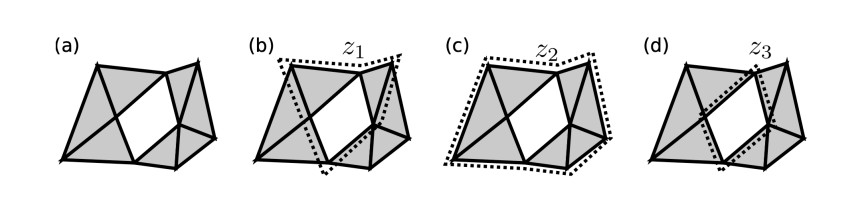
\includegraphics[width=0.8\textwidth]{images/homology_classes.png}
  \caption{Homology classes}
  \label{fig:homology_classes}
\end{figure}
\end{example}
\subsubsection{Устойчивая гомология}
Фильтрацию $F$ комплекса $K$ можно представить как вложенную последовательность подкомплексов:
\[\varnothing = K_0 \subset K_1 \subset \dots \subset K_m = K\]
Заметим, что эти вложенные комплексы могут возрастать скачками, то есть добавлять сразу множество симплексов. Чтобы это исправить, надо ввести порядок на этих симплексах:
\begin{definition}
  Пусть $F$ - фильтрация симплициального комплекса $K$. Введём на симплексах этого комплекса линейный порядок по:
  \begin{enumerate}
    \item Значению фильтрации
    \item Размеру симплекса
    \item Лексикографическому порядку вершин в симплексах
  \end{enumerate}

  Назовём позицией симплекса его номер в этом линейно-упорядоченном множестве. Заметим, что теперь можно представить фильтрацию комплекса как постепенное добавление симплексов в комплекс:
  \[\varnothing = \{\} \subset \{\sigma_1\} \subset \{\sigma_1, \sigma_2\}\subset \dots\subset \{\sigma_1, \dots,\sigma_n\} = K\]
  Для удобства обозначений, пусть $K_i := \{\sigma_1, \dots, \sigma_i\}$.
\end{definition}

Во время добавления нового симплекса $\sigma_i$ размерности $k$ к комплексу $K_{i-1}$ может произойти только одна из следующих вещей:
\begin{enumerate}
  \item $\sigma_i$ создаст новый гомологический класс
  \item $\sigma_i$ разрушит существующий гомологический класс
\end{enumerate}
Назовём симплекс позитивным или негативным соответственно. Заметим, что каждому негативному симплексу соответствует ровно один уникальный позитивный симплекс.
\begin{definition}
  Пара симплексов ($\sigma_i$, $\sigma_j$), где $i < j$, называется устойчивой, если добавление симплекса $\sigma_j$ в фильтрацию разрушило гомологический класс, который создало добавление симплекса $\sigma_i$.
\end{definition}
\begin{remark}
Если у позитивного симплекса не оказалось пары, его называют существенным, но такие симплексы нам не интересны.
\end{remark}
\subsubsection{Граничные матрицы}
\begin{definition}
  Гранью симплекса $\sigma$ называется любой $\tau\in K\colon \tau\subseteq \sigma$. Назовём грань с размерностью $\dim \tau = \dim \sigma - 1$ правильной гранью (\texttt{facet}). Границей симплекса называется множество его правильных граней.
\end{definition}
\begin{definition}
  Если $\tau$ - грань симплекса $\sigma$, то для $\tau$ симплекс $\sigma$ является когранью. Аналогично определяется правильная когрань (\texttt{cofacet}) и кограница симплекса.
\end{definition}
\begin{definition}
  Граничной матрицей фильтрации $F$ с $n$ симплексами называется бинарная квадратная матрица $M$ размера $n\times n$, где $M_{i,j}=1$ для каждой пары ($\sigma_i$, $\sigma_j$), если $\sigma_i$ является правильной гранью $\sigma_j$, и $M_{i,j}=0$ иначе.
\end{definition}
\begin{example}
  На рисунке~\ref{fig:boundary_matrix} подобие граничной матрицы для фильтрованного симплициального комплекса

\begin{figure}[ht]
  \centering
  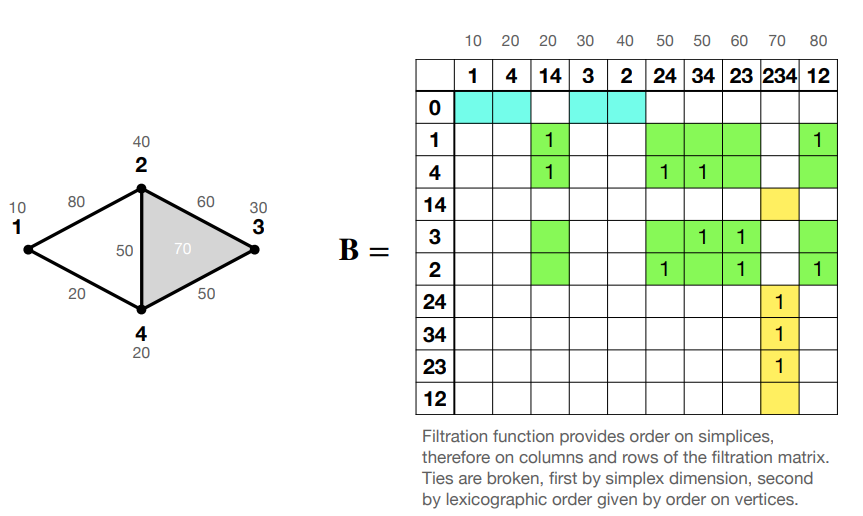
\includegraphics[width=0.8\textwidth]{images/boundary_matrix.png}
  \caption{Boundary matrix}
  \label{fig:boundary_matrix}
\end{figure}
\end{example}
Из граничной матрицы мы можем получить позиции устойчивых пар с помощью её редуцирования. Рассмотрим различные способы её редуцирования.
\begin{definition}
  Пусть $M_j$ - $j$ столбец граничной матрицы $M$. Назовём нижней позицией в этом слобце:
  \[\mathop{\rm low}(M_j) := \max\{i \in 1,\dots,n\colon M_{i,j} = 1\}\]
\end{definition}
Наивный способ редуцирования предполагает метод Гаусса на колонках граничной матрицы, т.е.

\begin{algorithm}[H]
\caption{Standard Reduction}
\KwIn{Граничная матрица $M$ с $n$ колонками}
\KwOut{Редуцированная граничная матрица $M$}
$L \gets [0,\dots,0]$ размера $n$ \tcp{в $L[i]$ мы храним индекс столбца $j$, для которого $\mathop{\rm low}(M_j) = i$}

\For{$j \in 1..n$} {
  \While{$M_j\neq 0$ and $L[\mathop{\rm low}(M_j)]\neq0$} {
    $M_j \gets M_j + M_{L[\mathop{\rm low}(M_j)]}$ \tcp{выполняется в поле $\Z_2$}
  }
  \If{$M_j\neq 0$} {
    $L[\mathop{\rm low}(M_j)] \gets j$
  }
}

\Return{M}
\end{algorithm}
\begin{lemma}
  Пусть $M$ - редуцированная граничная матрица. Тогда каждый ненулевой столбец в ней указывает на индексы симплексов в устойчивых парах, т.е.
  \[\{(i, j)\colon i = \mathop{\rm low}(M_j) \text{ and } M_j\neq 0\} \Leftrightarrow (\sigma_i, \sigma_j) \text{ является устойчивой парой}\]
\end{lemma}
\begin{example}
  Пример редуцирования фильтрованного 1-скелета можно увидеть на рисунке~\ref{fig:standard_reduction}. Получаем следующие устойчивые пары: [($\sigma_2$,$\sigma_4$), ($\sigma_1$, $\sigma_4$), ($\sigma_3$, $\sigma_6$)].

  \begin{figure}[ht]
    \centering
    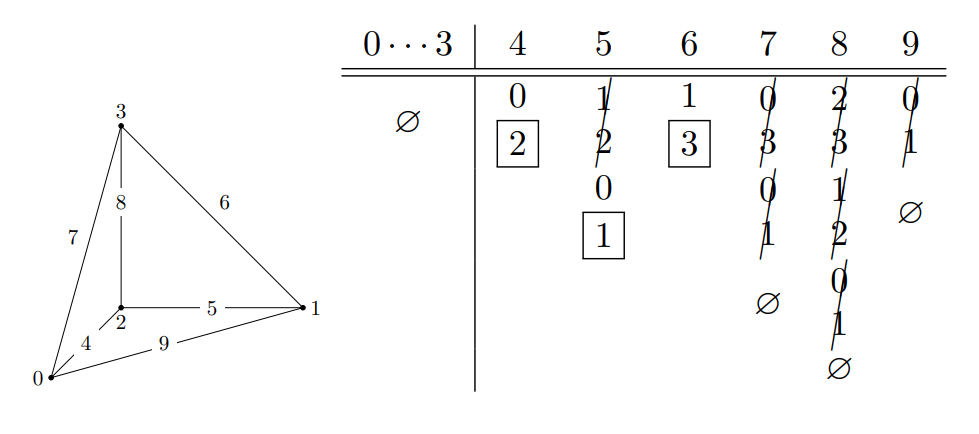
\includegraphics[width=0.8\textwidth]{images/standard_reduction.png}
    \caption{Standard reduction}
    \label{fig:standard_reduction}
  \end{figure}
\end{example}
\subsubsection{Twist}
\begin{lemma}
  Пусть $M$ - редуцированная граничная матрица фильтрации симплексов $[\sigma_1,\dots,\sigma_n]$. Тогда каждая колонка, которая соответствует позитивному симплексу в этой фильтрации нулевая.
\end{lemma}
Значит, если сначала средуцировать колонки, отвечающие за $(p+1)$-симплексы, то их нижние позиции будут указывать на позиции столбцов $p$-симплексов, которые можно занулить без длительного редуцирования:

\begin{algorithm}[H]
\caption{Twist Reduction}
\KwIn{Граничная матрица $M$ с $n$ колонками, максимальная размерность симплекса в фильтрации $d$}
\KwOut{Редуцированная граничная матрица $M$}
$L \gets [0,\dots,0]$ размера $n$ \tcp{в $L[i]$ мы храним индекс столбца $j$, для которого $\mathop{\rm low}(M_j) = i$}

$C \gets$ структура данных для быстрого получения $\mathop{\rm low}(C)$

\For{$\delta \in d..1$} {
  \For{$j \in 1..n$} {
    \If{$\dim \sigma_j \neq \delta$} {
      continue
    }

    $C \gets M_j$

    \While{$C\neq 0$ and $L[\mathop{\rm low}(C)]\neq0$} {
      $C \gets C + M_{L[\mathop{\rm low}(C)]}$ \tcp{выполняется в поле $\Z_2$}
    }

    \If{$C\neq 0$} {
      $L[\mathop{\rm low}(M_j)] \gets j$

      $M_{\mathop{\rm low}(C)} \gets 0$ \tcp{killing}
    }

    $M_j \gets C$
  }
}

\Return{M}
\end{algorithm}

В алгоритме также используетс структура данных для быстрого получения максимальной позиции в колонке. Для этой задачи подойдёт \texttt{BitTree}.

\subsubsection{BitTree}
Дерево представлено в виде кучи из массива 64 битных блоков. Уровни дерева:
\begin{itemize}
  \item Родительские узлы: блоки, где бит $i$ указывает на наличие дочерних элементов в поддереве $i$.
  \item Листья: блоки, хранящие битовые маски позиций (уровень 0).
\end{itemize} 
Опишем два главных алгоритма:

\begin{algorithm}[H]
\caption{Поиск максимальной позиции}
\KwIn{Поля \texttt{BitTree}}
\KwOut{Позиция старшего установленного бита}
\If{$\texttt{data\_[0]} = 0$} { \tcp{Дерево пусто - из корня нет рёбер}
    \Return UnknownPos
}

$node \gets 0$

$index \gets 0$

\While{true}{
    $block \gets \texttt{data}[node]$

    $index \gets \mathop{\rm RightmostBit}{(block)}$

    $next\_node \gets  (node \times 64) + index + 1$

    \If{$next\_node \geq |\texttt{data}|$}{
        Break
    }

    $node \gets next\_node$
}
$pos \gets (node - \text{offset}) \times 64 + index$

\Return $pos$
\end{algorithm}

Поиск $\mathop{\rm RightmostBit}{(block)}$ выполняется с помощью битхака \autocite{bithacks}

\[\mathop{\rm RightmostBit}{(block)} := 63 - \text{DeBruijn}_{64}\left[ (block \ \& -block) \cdot C \gg 58 \right]\]

где $C$ = 0x07EDD5E59A4E28C2 — константа для 64-битной де Брёйновой последовательности.

\begin{algorithm}[H]
\caption{Обновление бита для позиции (Xor)}
\KwIn{Позиция $pos$}
$block\_idx \gets \left\lfloor \frac{pos}{64} \right\rfloor$

$bit\_idx \gets 63 - (pos \mod 64)$

$mask \gets 1 \ll bit\_idx$

$\texttt{data}[block\_idx + \text{offset}] \gets \texttt{data}[block\_idx + \text{offset}] \oplus mask$

\While{$block\_idx > 0$}{
    $parent\_block \gets \left\lfloor \frac{block\_idx - 1}{64} \right\rfloor$

    $parent\_bit \gets (block\_idx - 1) \mod 64$

    $parent\_mask \gets 1 \ll (63 - parent\_bit)$

    $\texttt{data}[parent\_block + \text{offset}] \gets \texttt{data}[parent\_block + \text{offset}] \oplus parent\_mask$

    $block\_idx \gets parent\_block$
}
\end{algorithm}

\subsubsection{DoubleTwist}
Заметим, что если мы исследуем полные $k$-скелеты, то симплексов больших размерностей будет намного больше, чем малых, поэтому техника \texttt{Twist} неэффективна в таком случае. На помощь нам приходят когомологии.

Введём нотацию $i^\star = n - 1 - i$, где $n$ - общее количество симплексов.
\begin{definition}
  Кограничной матрицей фильтрации $F$ с $n$ симплексами называется бинарная квадратная матрица $M$ размера $n\times n$, где $M_{i^\star,j^\star}=1$ для каждой пары ($\sigma_{i^\star}$, $\sigma_{j^\star}$), если $\sigma_{i^\star}$ является правильной когранью $\sigma_{j^\star}$, и $M_{i^\star,j^\star}=0$ иначе.
\end{definition}

\begin{lemma}
  Если $j^\star$ является максимальной позицией к столбце $i^\star$ в редуцированной кограничной матрице, то  ($\sigma_{i^\star}$, $\sigma_{j^\star}$) - устойчивая пара.  
\end{lemma}

Заметим, что это отличается от случая граничной матрицы, где если бы $j$ была максимальной позицией в колонке $i$, то ей соответствовала бы устойчивая пара ($\sigma_{j}$, $\sigma_{i}$).

\begin{lemma}
  Аналогично граничному случаю, если $j^\star$ максимальная позиция непустого столбца $i^\star$, то можно занулить столбец $j^\star$.
\end{lemma}

Так как симплекс столбца $j^\star$ имеет большую размерность, чем симплекс столбца $i^\star$, то мы можем занулять столбцы симплексов больших размерностей, редуцируя сначала симплексы малых размерностей.

Получив редуцированную кограничную матрицу, нам надо отфильтровать столбцы граничной матрицы, чтобы получить все устойчивые пары. Фильтрация происходит следующим образом:

\begin{algorithm}[H]
\caption{Saving technique}
\KwIn{Редуцированная кограничная матрица $M$ размера $n$}
\KwOut{Позиции отфильтрованных столбцов}
$S \gets \varnothing$

\For{$j^\star \in 1..n$} {
  \If{$M_{j^\star} \neq 0$} {
    $S \gets S \cup \{\mathop{\rm Low}(M_{j^\star})\}$
  }
}

\Return $S$
\end{algorithm}

Затем мы конструируем граничную матрицу, где ненулевыми столбцами могут быть только сохранённые позиции. Далее редуцируем её как обычно.

\begin{lemma}
  Редуцированная граничная матрица, полученная с помощью техники \texttt{DoubleTwist} совпадает с матрицей, редуцированной с помощью обычных методов (метод Гаусса, \texttt{Twist}).
\end{lemma}

Опишем весь алгоритм целиком:

\begin{algorithm}[H]
\caption{DoubleTwist Reduction}
\KwIn{Фильтрация $F$ размера $n$}
\KwOut{Редуцированная граничная матрица $M$}
$M \gets \mathop{\rm CoboundaryMatrix}(F)$

reduce $M$ \tcp{например, с помощью \texttt{Twist}, но с возрастающим обходом размерностей}

$S \gets \mathop{\rm SavedPoses}(M)$

delete $M$ from memory

$B \gets \varnothing$

\ForEach{$i \in S$} {
  $B[i] \gets \mathop{\rm Boundary}(\sigma_i)$
}

reduce $B$

\Return $B$
\end{algorithm}

Остался вопрос, как быстро посчитать кограничную матрицу.

Можно заметить, что кограничная матрица является анти-транспонированной граничной матрицей. Но постройка и анти-транспонирование граничной матрицы намного медленнее, чем построение её с нуля.

Здесь появляется проблема: чтобы построить кограничную матрицу, надо быстро получать позиции правильных кограней симплексов в фильтрации.

Одним из решений будет генерировать всевозможные правильные кограни симплекса, но тогда появляется другая проблема: как проверить, что полученная когрань присутствует в фильтрации? Данная проблема не возникала с гранями, так как в симплициальном комплексе присутствуют все подсимплексы всех симплексов.

\subsubsection{SimplexTree}
Для решения этой проблемы была использована структура данных под названием \texttt{SimplexTree}. Это древовидная структура для представления симплициальных комплексов. Каждый узел соответствует вершине симплекса, а путь от корня к узлу представляет собой симплекс. Есть два уровня:
\begin{itemize}
  \item Корневой, где располагаются симплексы, представляющие собой вершины. Обычно представлен в виде массива указателей на следующий слой.
  \item Не корневой, представляет собой отдельные узлы дерева
\end{itemize}

В узлах дерева дополнительно хранится позиция симплекса, который представляет данный узел, в фильтрации, для быстрого и удобного получения позиции по номерам вершин симплекса.

Также, дерево поддерживает для каждой глубины дерева словарь списков, используемый для ускорения операций с ко-гранями. В списках хранятся все узлы дерева с заданной вершиной на данной глубине. Структура позволяет быстро находить все узлы определённого уровня, содержащие заданную вершину.

Опишем основные методы класса:

\begin{algorithm}[H]
\caption{Добавление симплекса}
\KwIn{Отсортированный симплекс $S = \{v_1, v_2, \dots, v_k\}$, его позиция в фильтрации $pos$}
\KwOut{Обновленное дерево}
$current \gets null$
$depth \gets 1$

\ForEach{$v_i \in S$}{
    \eIf{$current = null$}{
        $next \gets root[v_i]$
    }{
        $next \gets current.next[v_i]$
    }

    \If{$next$ не существует}{
        $next \gets$ Новый узел с родителем $current$ и вершиной $v_i$

        Связать узел в списке уровня глубины $depth$ и вершиной $v_i$
    }

    $current \gets next$

    $depth \gets depth + 1$
}

\If{$current != null$} {
  $current.pos \gets pos$
}
\end{algorithm}

\begin{algorithm}[H]
\caption{Получение позиций кограней}
\KwIn{Отсортированный симплекс $S = \{v_1, v_2, \dots, v_k\}$}
\KwOut{Множество позиций кограней}
$cofacets \gets \emptyset$

\If{$k = 0$}{
    \Return все корневые узлы
}

$base \gets \mathop{\rm Find}(S)$

\If{$base = \text{null}$}{
    \Return $cofacets$
}

\ForEach{$child \in base.next$}{
    $cofacets \gets cofacets \cup child.pos$
}

$list \gets $ Список нод на уровне $k+1$ для вершины $v_k$

\ForEach{$node \in list$} {
    \If{$node$ содержит $base$ как подсимплекс с 1 пропуском}{
        $cofacets \gets cofacets \cup node.pos$
    }
}

\Return $cofacets$
\end{algorithm}

\subsubsection{Промежуточные итоги}
Подводя итог, с помощью редуцированная граничной матрицы мы получили позиции пар устойчивых симплексов, которые все вместе составляют диаграмму устойчивости. В разной литературе под диаграммой устойчивости подразумевают пары значения фильтрации симплексов, а не их позиции в фильтрации, но
\begin{itemize}
  \item Можно легко перевести их в пары значений фильтрации по позициям в фильтрованном симплициальном комплексе
  \item Нам нужны именно позиции рождения и смерти для следующего шага
\end{itemize}
\subsection{Гармонические представители}
\subsubsection{Постановка задачи}
Устойчивая гомология примененяется к анализу мозговых сетей для определения формы мозговых сетей при различных пороговых значениях. Для измерения различий в сетях был предложен новый метод, а именно, использование гармонических дыр, которые выделяют подструктуры сетей мозга. Результаты показали, что эффективность кластеризации по гармоническим дырам выше, чем у сетевых расстояний, основанных только на глобальном изменении топологии.

Возникает задача быстрого вычисления всех гармонических дыр, полезных для выделения подструктур мозга. Но сначала надо ввести их определение.
\subsubsection{Матрица Ходжа-Лапласа}
\begin{definition}
  Пусть граничный оператор $\delta_k$ отобразил цепь из $k$-симплекса $[v_1,\dots, v_n]$ в сумму его правильных граней:
  \[\delta_k(\{\sigma_k\}) = \sum_{j=1}^k(-1)^{j-1}[v_1,\dots,\hat{v_j},\dots,v_k]\]
  Тогда полученные грани называются положительно/отрицательно ориентированными относительно симплекса $\sigma_k$.
\end{definition}
\begin{definition}
 Ориентированной граничной матрицей фильтрации $F$ с $n$ симплексами называется квадратная матрица $M$ размера $n\times n$, где $M_{i,j}=\pm 1$ для каждой пары ($\sigma_i$, $\sigma_j$), если $\sigma_i$ является правильной гранью $\sigma_j$, и $M_{i,j}=0$ иначе. Знак зависит от ориентации симплекса $\sigma_i$ относительно симплекса $\sigma_j$.
\end{definition}
Введём обозначения для подматриц ориентированной матрицы $M$:
\begin{itemize}
  \item $M_i$ - подматрица $M$, содержащая только столбцы, соответствующие $i$-симплексам фильтрации
  \item $M^k$ - подматрица $M$, содержащая столбцы $[1,\dots, k]\subseteq [1,\dots, n]$
  \item $M_i^k$ - комбинация верхних ограничений
\end{itemize}
\begin{definition}
   Комбинаторный Лапласиан Ходжа $L_i\colon C_i(K) \to C_i(K)$ определяется как:
   \[L_i := M_{i}^TM_i + M_{i+1}M_{i+1}^T\]

   Элементы $\ker L_i$ называют гармоническими циклами, а само ядро - гармоническим пространством $H_i$.
\end{definition}
\begin{lemma}
  $\mathop{\rm rk} H_i = \mathop{\rm rk} \tilde{H_i(K)}$
\end{lemma}
Таким образом, группу гомологий (обозначим её $\tilde{H_i(K)}$) можно заменить гармоническим пространством.

\subsubsection{Гармонические дырки}
\begin{definition}
Аналогично группе гомологий, в гармоническом пространстве $H_i$ присутствуют дырки, назовём их гармоническими дырками.
\end{definition}

Пусть у нас есть фильтрация 2-скелета симплициального комплекса с $p$ вершинами, $q$ рёбрами и $r$ треугольниками. Тогда $L_1\in \Z^{q\times q}$ и
\[H_1 = \{x\in \R^{q\times 1}\colon L_1 x = 0\}\]
Собственный вектор $L_1$ с нулевым собственным значением $x\in\R^{q\times 1}$ является представителем гармонической дырки. Абсолютное значение каждого элемента вектора $x$ представляет вес соответствующего ребра, то есть по появлению ребра в фильтрации.

Так как $x$ и $-x$ оба имеют нулевое собственное значение, то они представляют одну и ту же гармоническую дырку, и $||x|| = 1$.

\begin{example}
  Пусть мы получили собственный вектор $x$, представляющий некую гармоническую дырку. Отобразим его веса на рёбра как их толщину на рисунке~\ref{fig:harmonic_hole}.

  Явно можно наблюдать, что этот собственный вектор описывает дырку на вершинах 2, 3, 4, 6, 5. Остальные рёбра также имеют некий вес, но он мал по сравнению с весом рёбер описываемой дырки.

  \begin{figure}[ht]
    \centering
    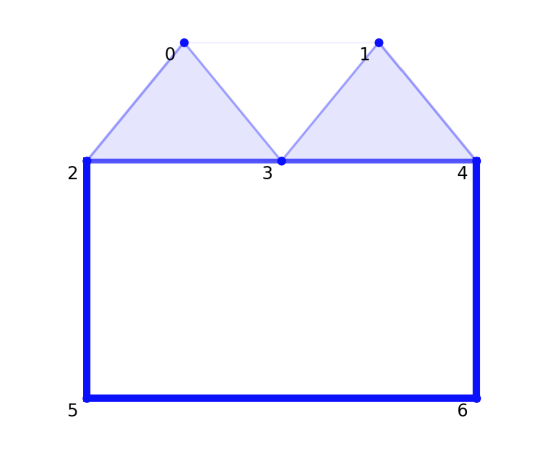
\includegraphics[width=0.5\textwidth]{images/harmonic_hole.png}
    \caption{Harmonic hole}
    \label{fig:harmonic_hole}
  \end{figure}
\end{example}

Но чтобы отследить все дырки, которые появлялись и исчезали во время фильтрации, пришлось бы вычислять ядро
\[L_1^k = (M_{1}^k)^TM_1^k + M_{2}^k(M_{2}^k)^T\]
для каждого момента фильтрации, от 1 до $n$, а это очень дорого из-за спектрального разложения. Поэтому, берут не все моменты фильтрации, а только моменты появления и исчезновения дырок, а это как раз и есть моменты из диаграммы устойчивости.
\subsubsection{Сепарация гармонических циклов}
Пусть мы рассматриваем пару из ($b_i$, $d_i$) - моменты рождения и смерти очередной дырки. При нахождении ядра матрицы Ходжа-Лапласа мы получаем множество из гармонических циклов. Для выделения представителя гармонической дырки рассмотрим следующий метод
\begin{enumerate}
  \item Пусть $i_X = b_i$, $i_Y = d_i - 1$, $i_Z = d_i$. $i_Y$ - это последний момент перед смертью дырки. Вычисляем гармоническое пространство для каждого из этих моментов фильтрации:
    \[H_X = [x_1,\dots,x_l]\in\R^{q\times l},\q H_Y = [y_1,\dots,y_m]\in\R^{q\times m},\q H_Z = [z_1,\dots,z_n]\in\R^{q\times n}\]
  \item Искомый представитель где-то в $H_X$ и $H_Y$, но не в $H_Z$
    \begin{lemma}
      Если $y\in H_Y$ линейно-зависим со столбцами $H_Z$, то минимальное сингулярное значение матрицы $[H_Z,y]$ будет близко к 0.
    \end{lemma}
    Так как существует $y\in H_Y$, линейно-независимый с $H_Z$, то мы выбираем $y$ как: 
    \[ y = \mathop{\rm argmax}\limits_{y\in H_Y}\{\sigma_{min} \text { of } [H_Z,y]\}\]
    Назовём его старшим представителем.

  \item Выберем младшего представителя как:
    \[x = \mathop{\rm argmin}\limits_{x\in H_X}\{\sigma_{min} \text { of } [x,y]\} = \mathop{\rm argmin}\limits_{x\in H_X}\left\{\sqrt{1 - |x^Ty|}\right\} = \mathop{\rm argmax}\limits_{x\in H_X}\{|x^Ty|\}\]
\end{enumerate}
Получаем для каждой гармонической дырки два представителя.
\subsubsection{Использование результатов}
Полученные на рёбрах веса можно агрегировать на вершины, складывая веса инцидентных рёбер или применяя другую функцию.

Далее, полученных представителей используют для подсчёта сетевых расстояний или дифференциации гармонический дырок. Также, к полученным данным применяются методы машинного обучения для дальнейшей идентификации и кластеризации гармонических дыр, но это выходит за рамки данной работы.
\section{Дизайн решения}
\subsection{Структурная диаграмма классов}

\begin{figure}[ht]
  \centering
  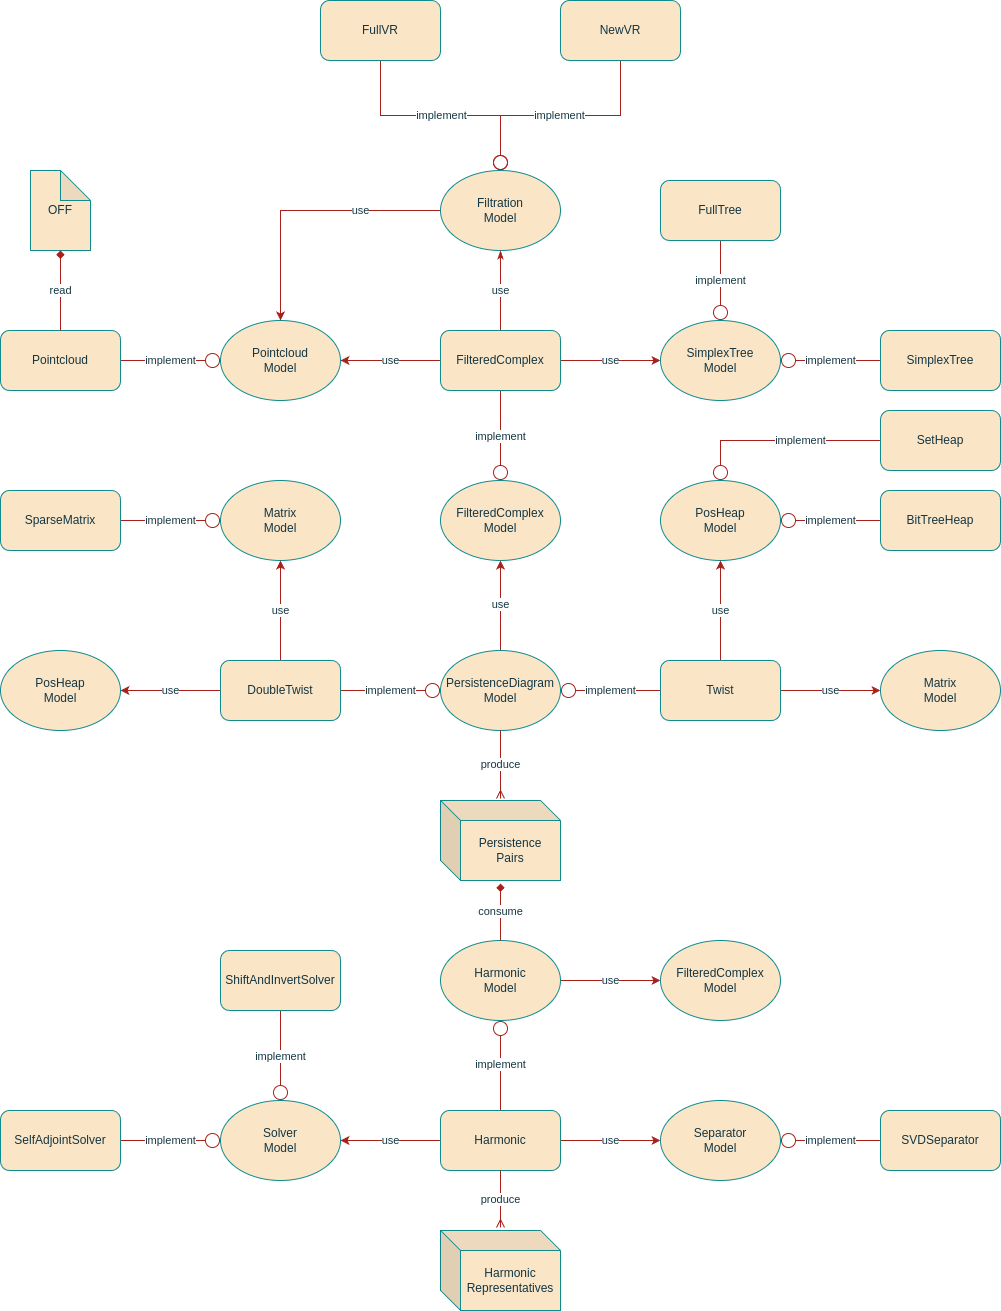
\includegraphics[width=0.75\textwidth]{images/class_diagram.png}
  \caption{Class Diagram}
  \label{fig:class_diagram}
\end{figure}
\clearpage

\subsubsection*{Описание потока данных}

\begin{enumerate}
  \item data.off $\rightarrow$ Pointcloud: Файл с набором точек считывается в облако точек
  \item Pointcloud $\rightarrow$ Filtration: Облако точек преобразуется в фильтрацию (например, полный комплекс Вьеториса-Рипса)
  \item Filtration $\rightarrow$ FilteredComplex: Симплексы сортируются и сохраняются в структуру данных
  \item FilteredComplex $\rightarrow$ PersistenceDiagram: Строится и редуцируется граничная матрица. По ней получаются устойчивые пары
  \item PersistenceDiagram $\rightarrow$ Harmonic: Пары передаются для анализа гармонических циклов
  \item Harmonic + Solver, Separator $\rightarrow$ HarmonicRepresentatives: Для каждой пары вычисляется её старший и младший представители
\end{enumerate}

\subsection{Модели и их реализации}
\begin{itemize}
\item \textbf{Pointcloud} — структура для хранения произвольно облака точек. Реализация позволяет считывать данные из файлов

\item \textbf{Filtration} — класс для построения фильтрации из облака точек. Генерирует симплексы и их значения фильтрации (например, полный 2-скелет комплекса Вьеториса-Рипса в \texttt{FullVR})

\item \textbf{SimplexTree} — структура для хранения симплексов и их позиций. Реализации: \texttt{FullTree} (для полного 2-скелета) и \texttt{SimplexTree} (для произвольного комплекса)

\item \textbf{FilteredComplex} — базовый класс для представления фильтрованного комплекса. Хранит симплексы с их позициями и предоставляет доступ к смежным элементам (граням и кограням). Используется для построения топологических структур

\item \textbf{Matrix} — абстракция для работы с разреженными матрицами (например, граничными операторами). Реализации: \texttt{SparseMatrix} на основе хеш-таблицы

\item \textbf{PosHeap} — структура данных для эффективного управления позициями в алгоритмах редукции. Реализации: \texttt{BitTreeHeap} (битовая куча) и \texttt{SetHeap} (на основе множества)

\item \textbf{PersistenceDiagram} — вычисляет устойчивые пары (рождение и смерть) на основе фильтрованного комплекса. Реализован в классах \texttt{Twist} и \texttt{DoubleTwist} через редукцию граничных матриц

\item \textbf{Solver} — решает задачу нахождения ядра матрицы. Реализации: \texttt{SelfAdjointSolver} (спектральное разложение для эрмитовых матриц) и \texttt{ShiftSolver} (использует метод Shift and Invert для разложения разреженных матриц)

\item \textbf{Separator} — решает задачу выделения линейно-независимого вектора из множеств векторов. Реализация \texttt{SVDSeparator} использует SVD разложение матриц для этих целей

\item \textbf{Harmonic} — вычисляет гармонические циклы, используя устойчивые пары. Интегрирует \texttt{Solver} и \texttt{Separator} для вычислений ядра и выделения линейно-независимых векторов соответсвтенно
\end{itemize}

\subsection{Ключевые алгоритмы}
\begin{itemize}
\item \textbf{Фильтрация}

Фильтрация Вьеториса-Рипса из облака $n$ точек
\begin{itemize}
    \item \textbf{FullVR}: Сложность: $O(n^3)$; Память: $O(n^3)$
    \item \textbf{NewVR}: Пусть допустимые рёбра будут определятся по случайному графу Эрдёша-Реньи ($G(n, p),\q p \in [0, 1]$). Тогда сложность будет равна $O(np^{(d_{max} - 1)})$, тогда как в реализации GUDHI сложность при тех же вводных $O(np)$, где $n$ - количество вершин
\end{itemize}

\item \textbf{Дерево симплексов}
\begin{itemize}
  \item \textbf{SimplexTree}:
  \begin{enumerate}
    \item \textbf{Add}, \textbf{Has}, \textbf{GetPos}: Сложность $O(k\log m)$, где $k$ — размер симплекса, $m$ — среднее количество потомков узла
    \item \textbf{GetFacetsPos}: Сложность $O(k^2\log m)$
    \item \textbf{GetCofacetsPos (Sparse)}: Сложность $O(q)$, где $q$ - количество узлов на уровне $k + 1$
    \item \textbf{GetCofacetsPos (Dense)}: Сложность $O(nk)$
  \end{enumerate}
  \item \textbf{FullTree}:
  \begin{enumerate}
    \item \textbf{Add}, \textbf{Has}, \textbf{GetPos}: Сложность $O(1)$
    \item \textbf{GetFacetsPos}: Сложность $O(1)$
    \item \textbf{GetCofacetsPos}: Сложность $O(n)$, где $n$ - количество вершин
  \end{enumerate}
\end{itemize}

\item \textbf{Вычисление диаграммы устойчивости}:
\begin{itemize}
  \item \textbf{Twist}: Сложность $O(n + m)$, где $n$ - количество симплексов, а $m$ - количество ненулевых элементов в матрице
  \item \textbf{DoubleTwist}:  Сложность $O(n + m)$, но константа значительно меньше
\end{itemize}

\item \textbf{Вычисление гармонических циклов}:
\begin{itemize}
  \item \textbf{Фильтрация устойчивых пар}: $O(m\log m)$, где $m$ - количество пар
  \item \textbf{Построенние ориентированной граничной матрицы}: $O(n)$
  \item \textbf{Вычисление Лапласиана}: $O(nnz)$, где $nnz$ - количество ненулевых элементов в матрицах $B_0$ и $B_1$
  \item \textbf{Поиск ядра лапласиана}: $O(kn^2)$, где $k$ - число итераций в методе Shift-and-Invert, $n$ - размер матрицы
  \item \textbf{SVD-разделение}: $O(m^3)$, где $m$ - число столбцов в матрице \texttt{basis}
  \item \textbf{Обновление циклов}: $O(k(e + v))$, где $k$ - число циклов, $e$ - рёбер, $v$ - вершин
\end{itemize}
Доминирующие шаги - решение спектральной задачи $O(kn^2)$ и SVD-разделение $O(m^3)$. Худший случай: $O(n^3)$.
\end{itemize}
\subsection{Тестирование}
Все классы и функции покрыты юнит и стресс тестами с помощью фреймворка Catch2 \autocite{catch2}. Проведены сравнительные бенчмарки для нахождения наилучших комбинаций из алгоритмов для поиска гармонических циклов.

Добавлены сравнительные бенчмарки с различными имплементациями других библиотек, а также построены их графики и добавлены в \href{https://github.com/Hackerman-ru/Topological-Analysis}{репозитории проекта}.
\newpage
\appendix
\section{Глоссарий}\label{glossary}
\begin{itemize}
  \item Симплициальный комплекс/комплекс - Подмножество $2^V$, замкнутое относительно взятия подмножеств. Состоит из симплексов.
  \item $k$-симплекс - Симплекс, содержащий $k+1$ вершину. Размерность $\dim\sigma = k$
  \item $i$-скелет - Подкомплекс комплекса $K$ содержащий все симплексы размерности $\leq i$
  \item Полный 2-скелет - Это комплекс, содержащий все возможные рёбра и треугольники (1- и 2-симплексы) между вершинами
  \item Фильтрация/фильтрованный комплекс/фильтрованный симплициальный комплекс - Упорядоченное семейство вложенных симплициальных комплексов $\{K_f\}_{f\in\R}$
  \item Граничный оператор - Линейный оператор $\delta_k\colon C_k(K)\to C_{k-1}(K)$, сопоставляющий симплексу сумму его граней с учётом ориентации
  \item Группа гомологий - Факторгруппа $H_k(K) = Z_k(K)/B_k(K)$, где $Z_k$ - циклы, $B_k$ - границы
  \item Когомологии — Двойственные к гомологиям структуры, где цепи рассматриваются как функции на симплексах
  \item Устойчивая пара - Пара симплексов ($\sigma_i$, $\sigma_j$), где добавление $\sigma_j$ уничтожает гомологический класс, созданный $\sigma_i$
  \item Гармонический цикл - Элемент ядра комбинаторного оператора Ходжа-Лапласа $L_i = \delta_i^*\delta_i + \delta_{i+1}\delta_{i+1}^*$
\end{itemize}
\newpage
% Здесь автоматически генерируется библиография. Первая команда задает стиль оформления библиографии, а вторая указывает на имя файла с расширением bib, в котором находится информация об источниках.
\addcontentsline{toc}{section}{Список литературы}
\printbibliography

% Здесь текст документа заканчивается
\end{document}
% Начиная с этого момента весь текст LaTeX игнорирует, можете вставлять любую абракадабру.

